\chapter{Proposed Methodology}\label{chap:method}

\section*{}

In order to help the patients and the physicians to define the best treatment plan and to choose the treatment that may result on the best aesthetic outcome for the patient offering her the best quality of life despite of the side-effects of the breast cancer treatment, the result of the Breast Conserving Surgery may be predicted.

In this chapter the method to obtain of the prediction models is described.

\section{Flowchart}

Figure \ref{fig:flowchart1} presents the flowchart with the phases on the proposed methodology.


\begin{figure}[H]
  \begin{center}
    \leavevmode
    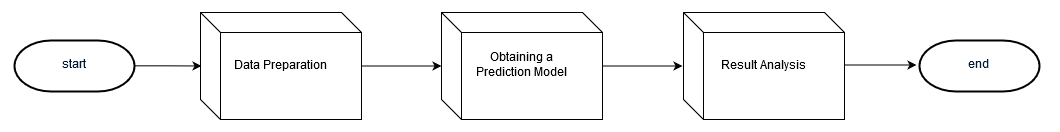
\includegraphics[width=1\textwidth]{flowchart1}
    \caption{Flowchart with methodology phases}
    \label{fig:flowchart1}
  \end{center}
\end{figure}

This methodology is shown in more depth in figure \ref{fig:flowchart2}. The methodology is present phase by phase on the next sections with a greater level of detail.

\begin{figure}[H]
  \begin{center}
    \leavevmode
    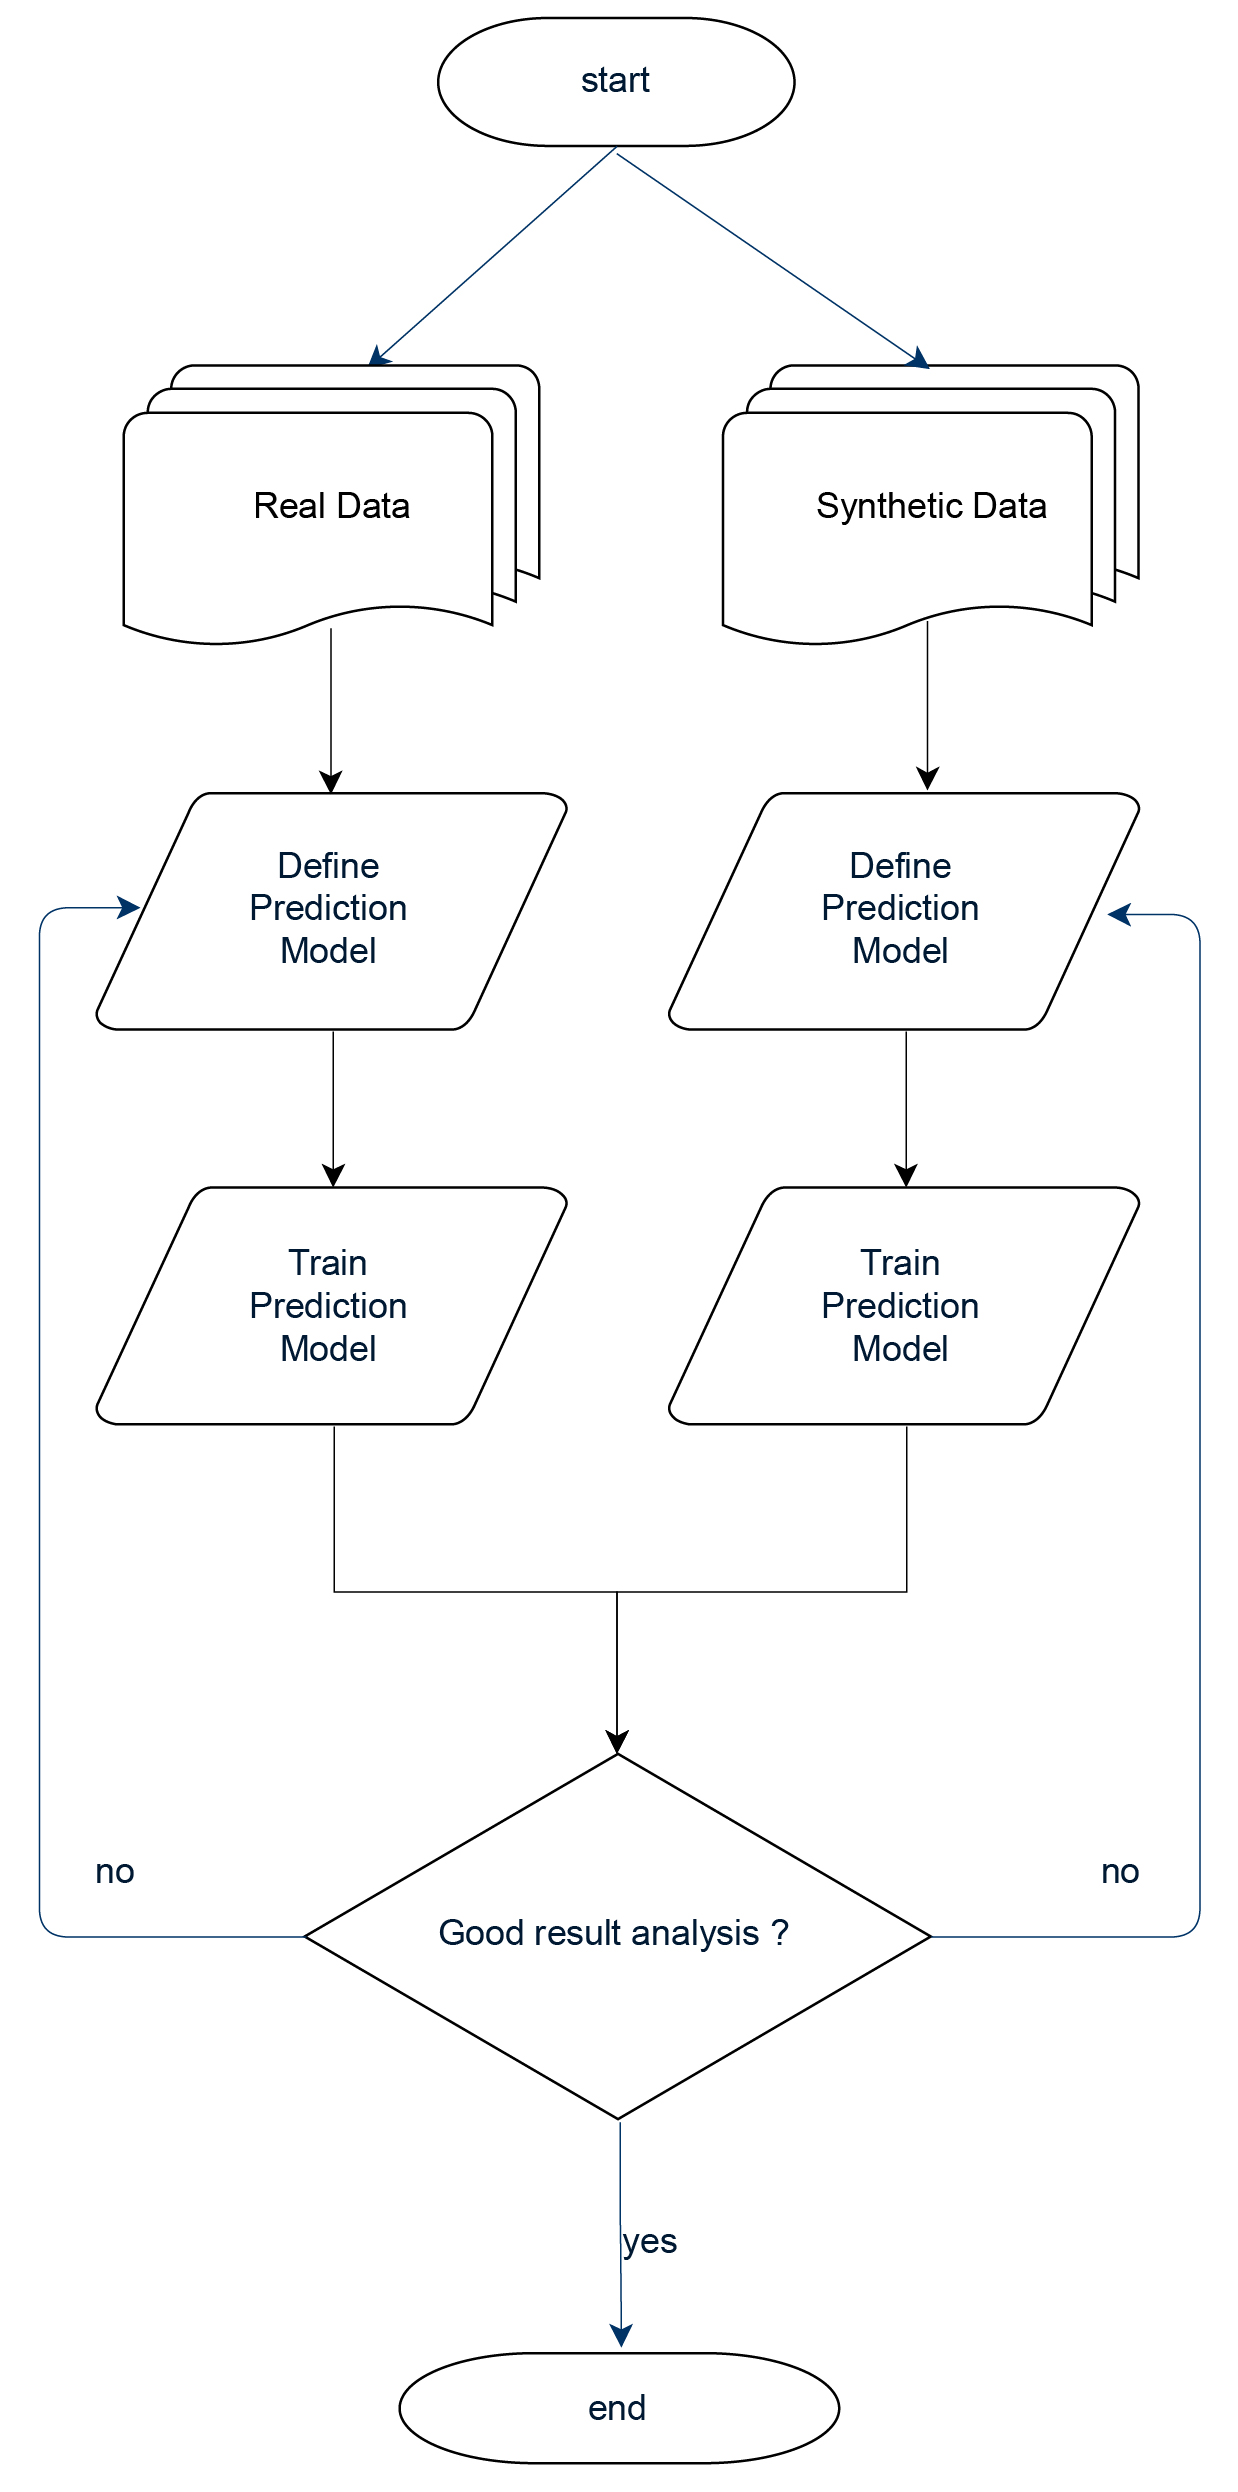
\includegraphics[width=0.6\textwidth]{flowchart}
    \caption{Flowchart with main tasks}
    \label{fig:flowchart2}
  \end{center}
\end{figure}

\clearpage

\section{Data preparation}

In order to produce better prediction results, the prediction model must consider a high number of cases and examples. The information regarding the 36 patients that INESC TEC have gathered is by far not enough so the creation of synthetic data based on the gathered cases is required.

The information already gathered counts with pre-surgery and post-surgery models of the patient's breast, and the respective medical annotations concerning the treatment that the patient has been under and some additional information.

On the information already gathered, there were used both surface extractor (kinect) and MRI information to model the breast of the patients. It can be used to describe the surface of the breast and MRI to describe the interior of the breast's model. The annotations were taken by health professionals and concern information regarding the following aspects:

\begin{itemize}
\item Breast Density
\item Laterality - Indicates if the tumor is positioned on the left or the right breast
\item Tumor Position - The position of the tumor is described according with the quadrant of the breast where it is located
\item Ptosis - Ptosis is a deformation that describes the sagging that affects the breast with aging.
\item Tumor Volume
\item Tumor Size
\end{itemize}

To produce the synthetic data, the same data for each patient is required: the pre-surgery and post-surgery models of the breast and the medical annotations. This generation of data must be done simultaneously. The breast models at this stage, must include which parts of the model are labeled as healthy tissue and which are labeled as damaged tissue.

\section{Obtaining a Prediction Model}
In order to obtain the prediction model, and recurring to the data previously gathered form real patients and the data previously synthesized, the prediction model may be firstly defined. As soon as a good definition of the model is achieved, the same prediction model may be implemented using Deep Neural Networks (DNN).

Deep neural networks can be seen as stack neural networks, a set of algorithms designed to recognize patterns. The neural network combines input from data that with different weight associated to each input layer lead to the result of the output layers.

Using DNN will allow to train the model taking into consideration the high variability of the shapes that the breast can take depending from patient to patient. This approach as been proved to retrieve good results when predicting aspects on diverse fields of expertise.

After the training of the model, a verification of the training can be done considering a 1-vs-all approach. This is the approach that makes more sense regarding once more the great variability of shapes that a breast's patient can take. This will also allow that the model will not suffer any overfitting despite the great amount of data used.

A refinement concerning the prediction model may be needed. This aspects shall be further though after the analyzes of the results that the first predictive model may produce.


\section{Result Analysis}

The Result analysis focus on two distinct aspects:

\begin{itemize}
\item Test and Validation of the Prediction Models
\item Analysis of aspects that may influence the Aesthetic Outcome
\end{itemize}

The validation and testing of the prediction models lays on the evaluation of several metrics. Some of the metrics that may be used can consider the euclidean distance between the real or synthesized post-surgery model and the predicted model given by the application of the prediction model on both the pre-surgery model (real or synthesized) and the medical annotations of the specific patient. Another comparison metric able to be use can be the difference on the volume changes of the models referred above. Any of this comparison can only be applied partially, once the overlaying of the models is a complex problem that was not been solved yet. 

Regarding the analysis of the features that influence the outcome of the surgery, that is a controversial and high discussed topic on clinical papers, the goal is to define which of those features may lead to a different aesthetic outcome and how much do they influence the surgery result on the breast conserving treatment.

\section{Work Plan}

The work plan is visible in figure \ref{fig:gantt} through a gantt chart.

The first tasks described is the preparation of data that includes the syntetization of data regarding the pre-surgery and post-surgery models of the breast and the annotations with the required parameters enumerated previously. All this subtasks may be done simultaneously.

The second task focus on obtaining a prediction model. In order to complete this, the prediction model may first be defined and then implemented. A refinement to this model may be necessary after the analyze of some of the results it will produce.

The third task refers to the result analysis, where the results of the prediction model may be analysis as well as the influence of the feature responsible for the model outcome may be measured.

Last but not least, the fourth tasks includes the thesis' report writing.

\begin{figure}[H]
  \begin{center}
    \leavevmode
    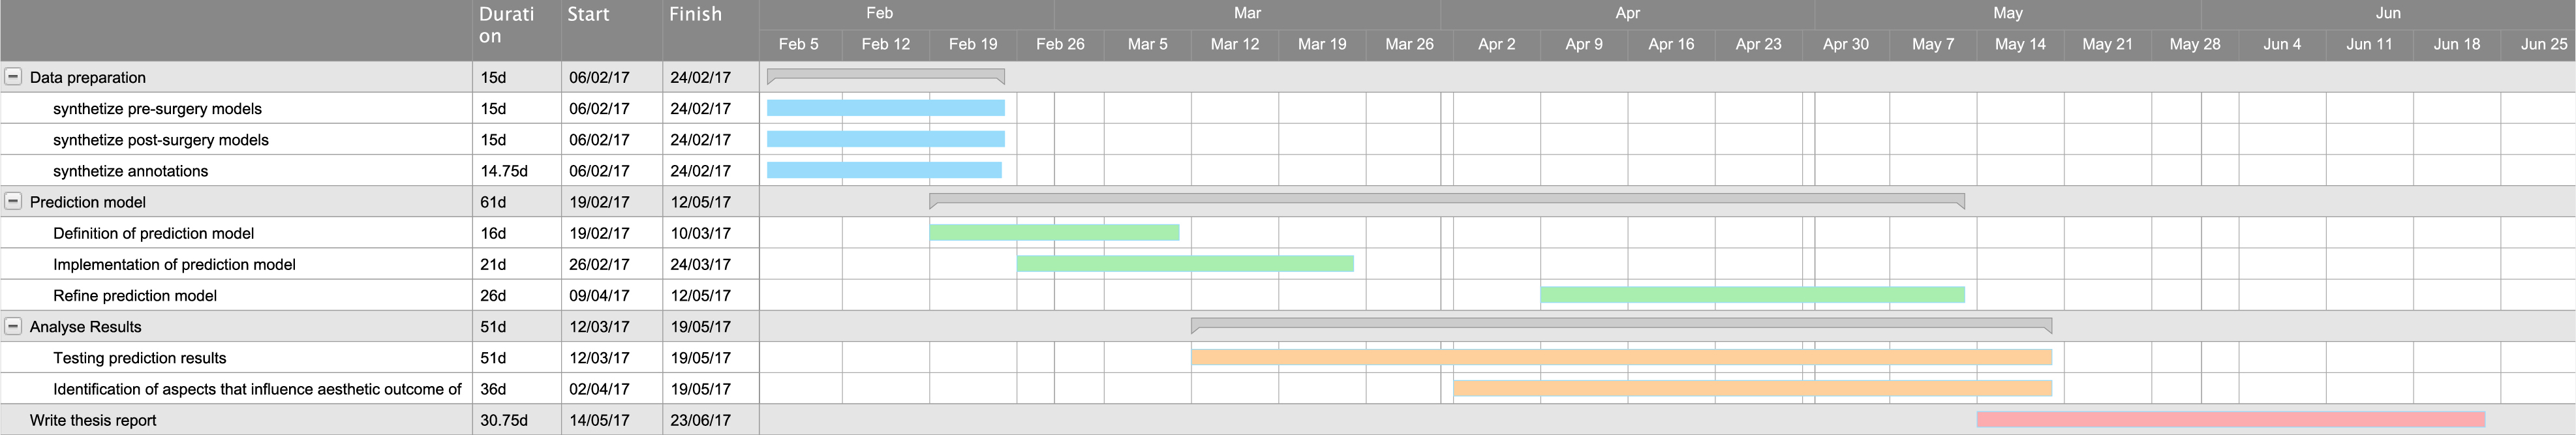
\includegraphics[width=1.4\textwidth, angle=-90]{gantt}
    \caption{Gantt Chart}
    \label{fig:gantt}
  \end{center}
\end{figure}


\section{Summary}

In this chapter, the steps to obtain the predictive model for breast deformation on BCCT are detailed. The major stages of the methodology: data preparation, obtainment of prediction model and analysis result were specified on this chapter. Some aspects may be defined during the methodology progress concerning the results obtained on the previous steps. The next chapters focus on the conclusions made so far regarding the proposed methodology and the presented state of the art described and present the work plan and the estimated time each stage and task will take is also presented on this chapter.
